%本文件内容为第五章:电路控制系统,本章一共分为?节
%本文件由徐哲编写
%本文件于1.10日修改

\chapter{机电控制系统}

\section{电机选型}

由本项目的结构设计可知,整体共有五个自由度,需要五个电机进行驱动。
鉴于机械臂及云台转动角度的精准度要求较高,本项目的机械臂部分均采用
步进电机进行驱动。而手部仅要求简单控制电机轴正反转即可,因此手部
选用直流有刷电机。

接下来将根据各个关节输入的需求,分析电机的选型。
~\\

\begin{enumerate}
\item \textbf{云台:}经过搜索,我们能买到的较大扭矩的步进电机(86步进电机,如图~\ref{fig:86})可以提供约
4$N\cdot M$的扭矩,经过与蜗轮蜗杆的配合减速,正常运行时能产生约200$N\cdot M$的
扭矩,以及约3.5转/分的转速,可以满足对云台的驱动要求。
\item \textbf{1号臂:}由于1号臂所承受的载荷最大,驱动1号臂需要的扭矩也较大,因此同样选择
与云台相同的大型86步进电机(4$N\cdot M$型),经过蜗轮蜗杆的配合减速,正常运行时能
产生约150$N\cdot M$的扭矩,经Matlab核算,可以满足1号臂的扭矩需要,减速后
的转速最快可至6转/分,也足够满足需求。
\item \textbf{2号臂:}由于2号臂与3号臂部分没有外加减速机构,因此选用电机时需要直接选用减速
电机增大输出扭矩,且本身体积与质量不能过大,否则对1号臂负担过大。经过
选择,2号臂最终采用了减速比1:99的42减速电机(0.7$N\cdot M$型,如图~\ref{fig:42}),减速后的
输出扭矩可达69.3$N\cdot M$,转速接近2转/分,可以满足2号臂的转动需要。
\item \textbf{3号臂:}3号臂与2号臂要求类似,只是需要的扭矩较2号臂小一些,因此采用扭矩为0.55$N\cdot M$,
减速比1:99的42减速电机,减速后的输出扭矩约为54.45$N\cdot M$,转速同样为2转/分,
可以满足3号臂的转动需要。
\item \textbf{手部:}根据上文中手部结构的设计,夹取时需要的输入扭矩大约为0.5$N\cdot M$,故选用了减速比
为1:142的直流减速电机(如图~\ref{fig:DCmotor}),其最终输出扭矩可达0.6$N\cdot M$,满速转速为30转/分,可以
满足手部输入的要求。
\end{enumerate}

~\\

综上,电机部分的选型如下:
\begin{minipage}[t]{0.9\linewidth}
  云台:86步进电机(4$N\cdot M$)
\\1号臂:86步进电机(4$N\cdot M$)
\\2号臂:42减速步进电机(69.3$N\cdot M$)
\\3号臂:42减速步进电机(54.45$N\cdot M$)
\\手部:直流减速有刷电机(0.6$N\cdot M$)
\end{minipage}
\\


    86步进电机型号:86BYG250B 
   
    转速:200转/分   \qquad \qquad 扭矩:4$N\cdot M$ \qquad \qquad 机身长度:80MM  
     
    轴径:14MM \qquad \qquad 电机电流:4A \qquad \qquad 出线:二相四线 
    \begin{figure}[!htp]
        \centering
          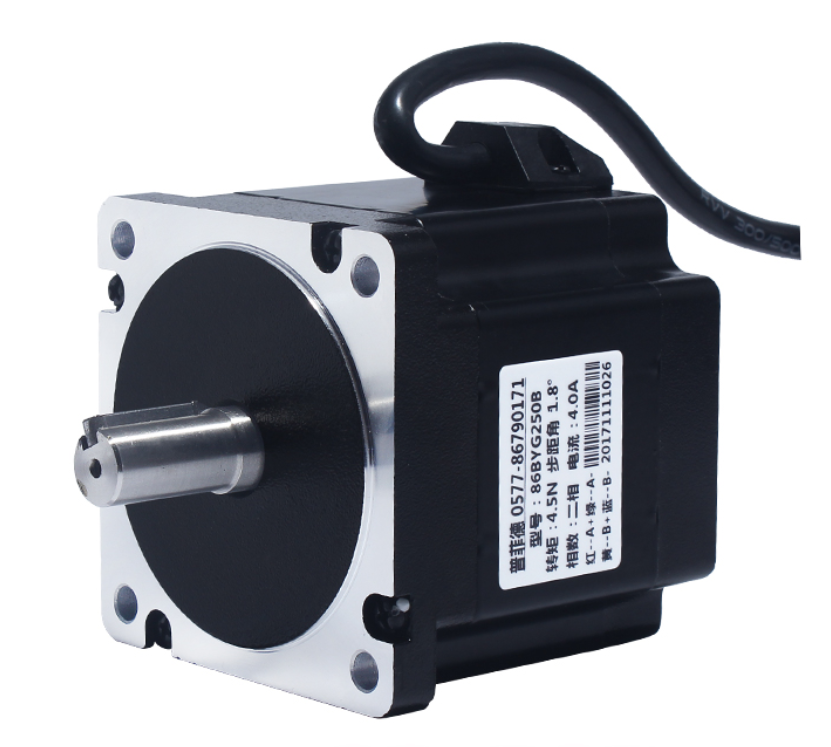
\includegraphics[height=5cm]{stepmotor86.png}
          \bicaption[86步进电机]{86步进电机}{Step motor: model 86}
          \label{fig:86}
    \end{figure}
~\\

    42步进电机型号:42BYGH47/42BYGH60
     
    转速:200转/分  \qquad  扭矩:0.55/0.7$N\cdot M$ \qquad  机身长度:48/60MM  \qquad 轴径:5MM
    
    电机电流:1.5A \qquad  出线:二相四线 \qquad  减速箱长度:48MM  \qquad  减速比:1:99
    \begin{figure}[!htp]
        \centering
        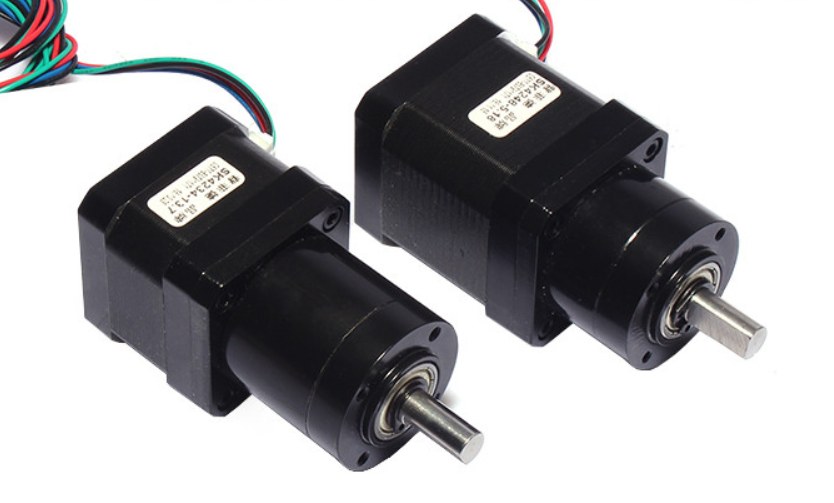
\includegraphics[height=5cm]{stepmotor42.png}
        \bicaption[42步进减速电机]{42步进减速电机}{Step motor: model 42}
        \label{fig:42}
    \end{figure}



        直流有刷电机型号:XD-37GB520(带减速箱)
        
        输入电压:DC12V \qquad 负载电流:0.68A \qquad 整体重量:约210g \qquad 额定功率:7W

        减速比:1:99 \qquad 减速箱长度:28MM \qquad  输出转速:30转/分 \quad  输出扭矩:0.6$N\cdot M$
        \begin{figure}[!htp]
        \centering
        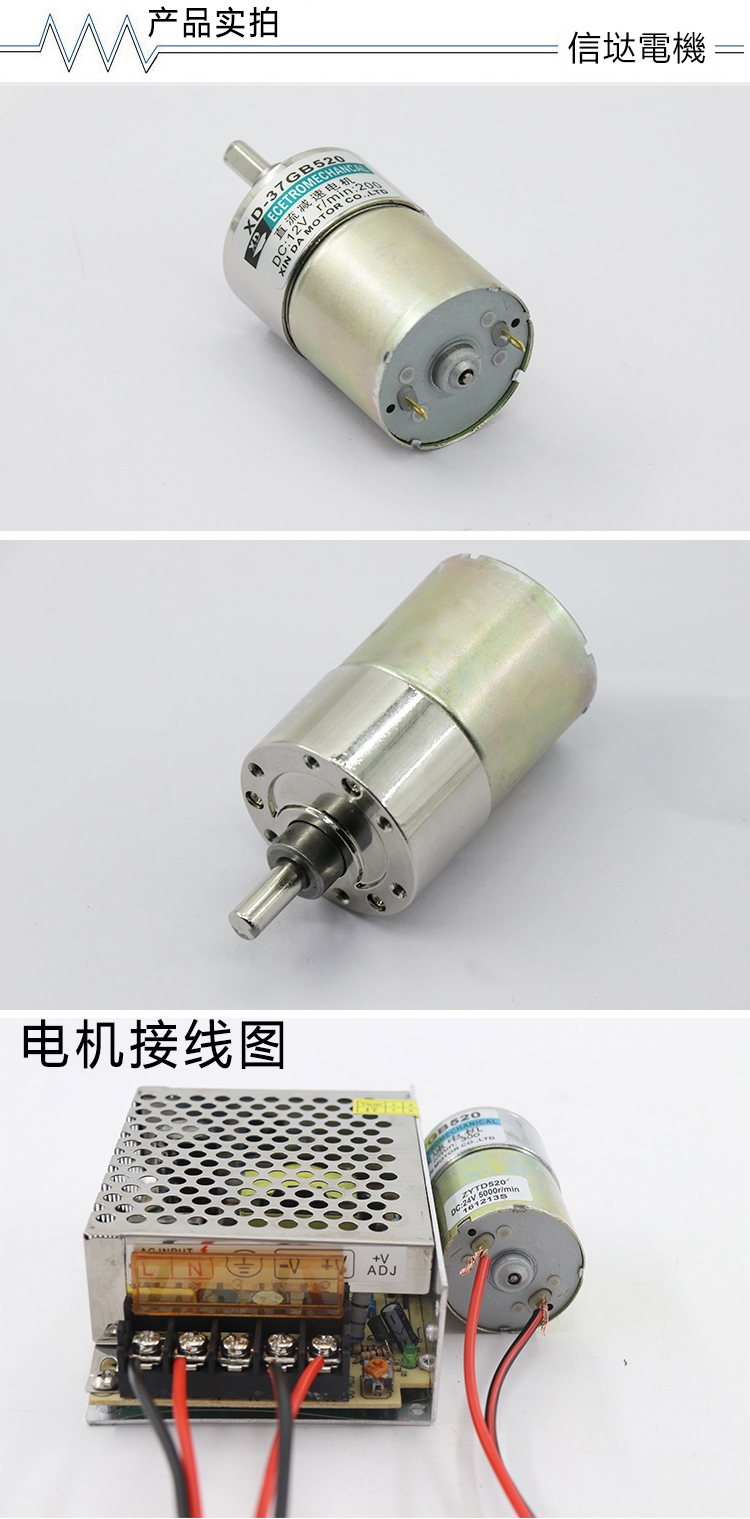
\includegraphics[height=5cm]{DCmotor.jpg}
        \bicaption[直流有刷电机]{直流有刷电机}{DC brush motor}
        \label{fig:DCmotor}
        \end{figure}
        
        
~\\

\section{驱动器选择}

\subsection{步进电机驱动}

86步进电机驱动器型号:DM542

具体参数:
\begin{minipage}[t]{09\linewidth}
    脉冲信号:3.3V/5V/24V兼容   \qquad
    输入电压:直流DC12V-50V

    细分设定:400-25600细分     \qquad \quad
    电流范围:1.0A-4.0A
\end{minipage}
\\

42步进电机驱动器型号:DM542C

具体参数:
\begin{minipage}[t]{09\linewidth}
    脉冲信号:3.3V/5V/24V兼容   \qquad
    输入电压:直流DC20V-50V

    细分设定:400-25600细分     \qquad \quad
    电流范围:1.0A-4.2A
\end{minipage}
\\

\subsection{直流电机驱动}

驱动器型号:L298N直流电机驱动芯片 \quad 蓝色版

具体参数:
\begin{minipage}[t]{09\linewidth}
    驱动电压范围Vs:+5V-35V    \qquad
    逻辑电压范围Vss:+5V-7V

    控制信号和使能信号电压:低电平-0.3V-1.5V  \quad
    高电平2.3V-Vss
\end{minipage}

\begin{figure}[!htp]
    \begin{minipage}{0.32\textwidth}
      \centering
      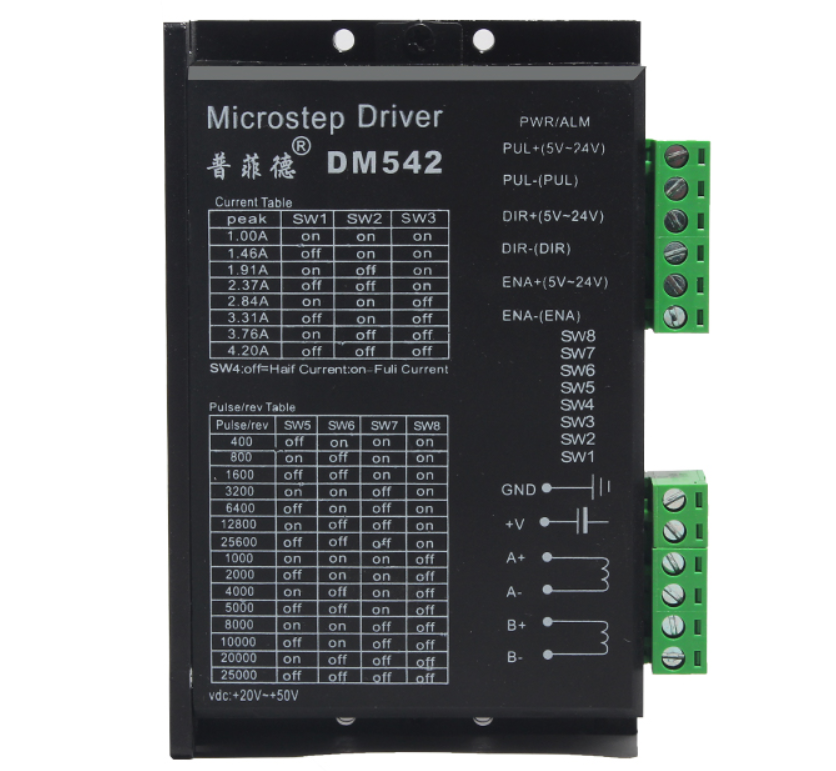
\includegraphics[height=3.5cm]{DM542.png}
      \bicaption[DM542]{DM542}{DM542}
      \label{fig:DM542}
    \end{minipage}\hfill
    \begin{minipage}{0.32\textwidth}
      \centering
      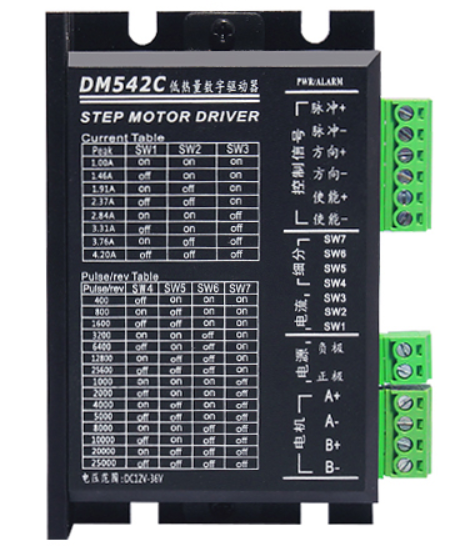
\includegraphics[height=3.5cm]{DM542C.png}
      \bicaption[DM542C]{DM542C}{DM542C}
      \label{fig:DM542C}
    \end{minipage}
    \begin{minipage}{0.32\textwidth}
      \centering
      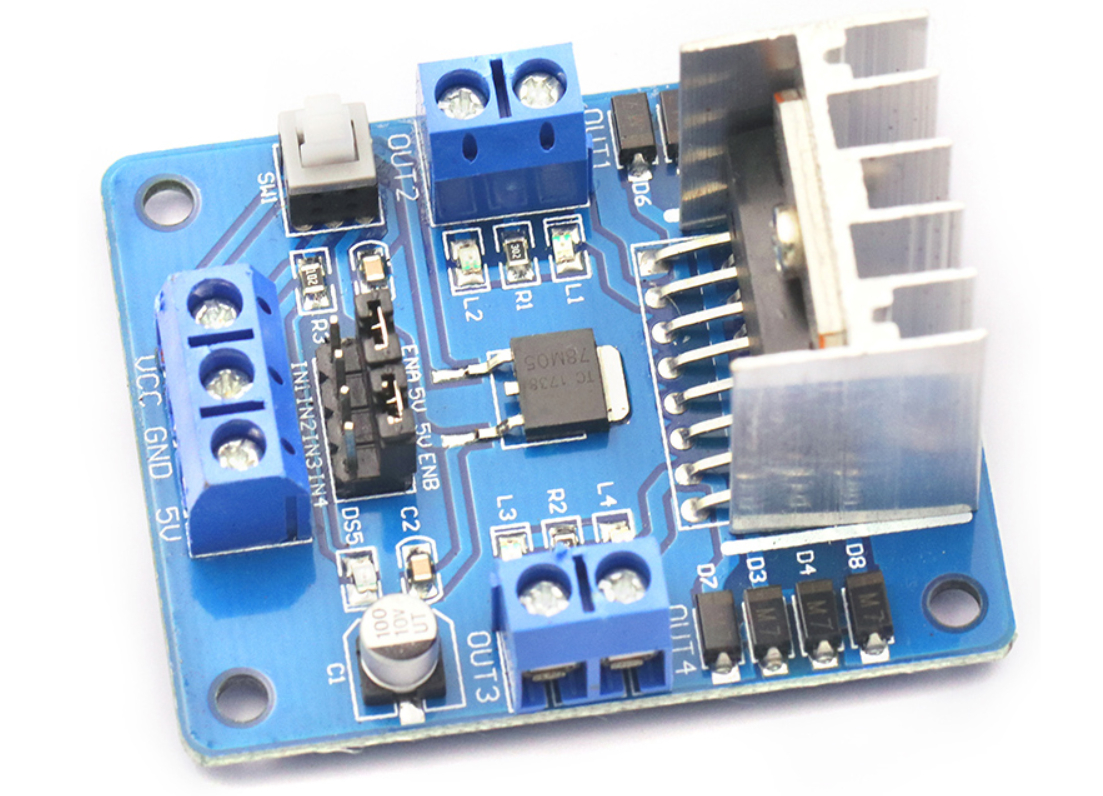
\includegraphics[height=3.5cm]{L298N.png}
      \bicaption[L298N]{L298N}{L298N}
      \label{fig:L298N}
    \end{minipage}
\end{figure}

\section{电源选择}

\subsection{供DM542驱动器}

产品型号:S-250W-24V

直流输出电压:24V  \qquad \qquad 输出电流:0-10A \qquad \qquad 输出功率:250W

\begin{figure}[!htp]
    \centering
    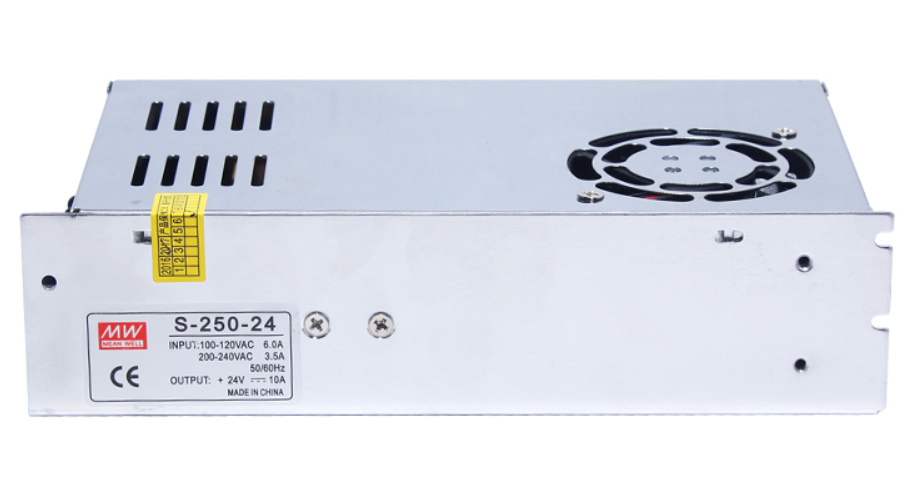
\includegraphics[height=5cm]{powersource250w.png}
    \bicaption[250W电源]{250W电源}{250W source}
    \label{fig:250W}
\end{figure}

\subsection{供DM542C驱动器}

产品型号:S-100W-24V

直流输出电压:24V  \qquad \qquad 输出电流:0-4.2A \qquad \qquad 输出功率:100W
\begin{figure}[!htp]
    \centering
    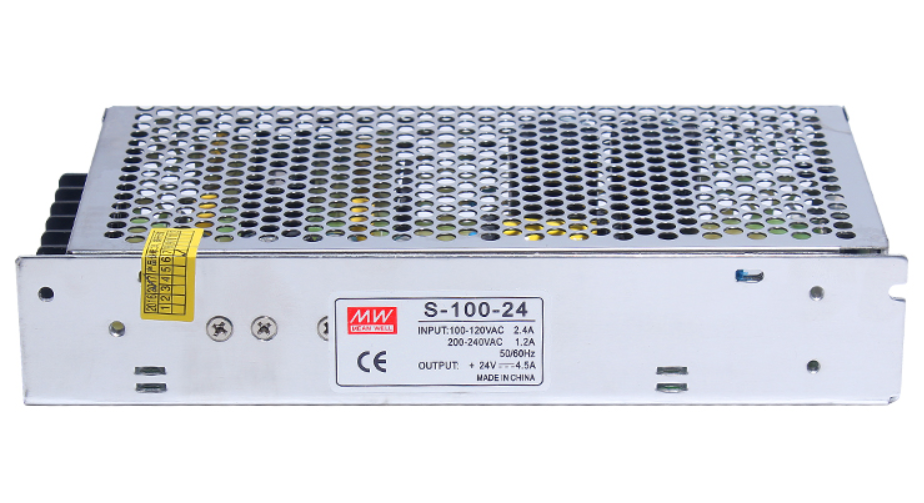
\includegraphics[height=5cm]{powersource100.png}
    \bicaption[100W电源]{100W电源}{100W source}
    \label{fig:100W}
\end{figure}
\begin{figure}[!htp]
    \centering
    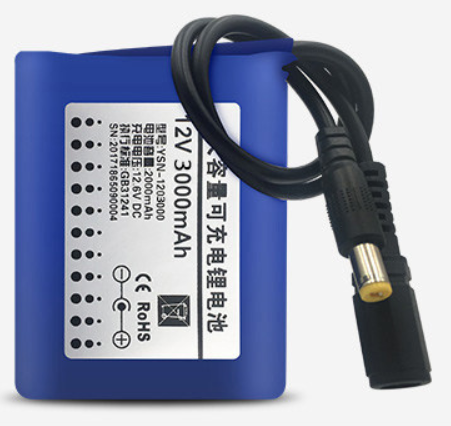
\includegraphics[height=5cm]{powersource12v.png}
    \bicaption[12V电源]{12V电源}{12V source}
    \label{fig:12V}
\end{figure}
\subsection{供L298N驱动器}

产品型号:YSN-1203000锂电池组

直流输出电压:12V

\section{传感器选择}

本项目仅有手部需要传感器进行夹取力度的控制,考虑到对传感器有尺寸小、质量轻、灵敏度高
等要求,最终选用了薄膜式压力传感器,将其固定于抓手内侧。

传感器型号:RP-C7.6-ST \qquad 外径:7mm \qquad 量程范围:2g-1.5kg
\begin{figure}[!htp]
    \centering
    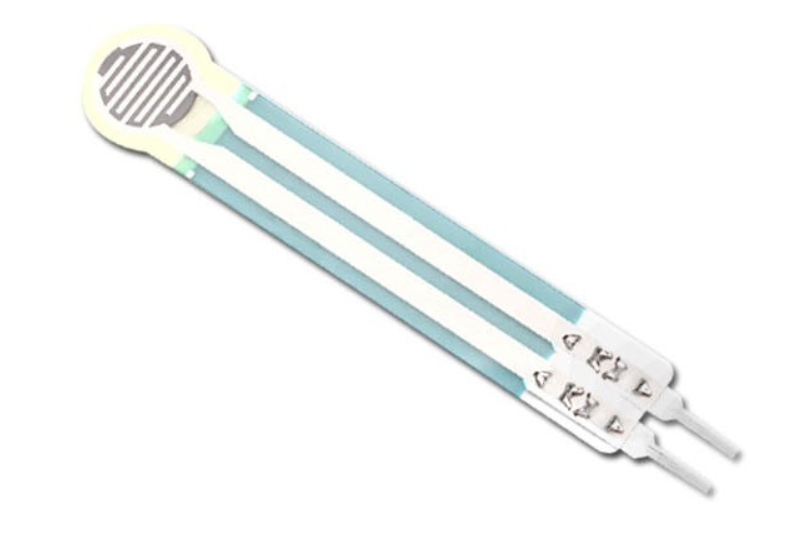
\includegraphics[height=5cm]{forcesensor.png}
    \bicaption[压力传感器]{压力传感器}{Pressure sensor}
    \label{fig:压力传感器}
\end{figure}
\section{控制板选择}

本项目选用arduino UNO作为机电系统的控制板,其输出端口数量与数据处理能力
足够满足本项目需求。

\begin{figure}[!htp]
    \centering
    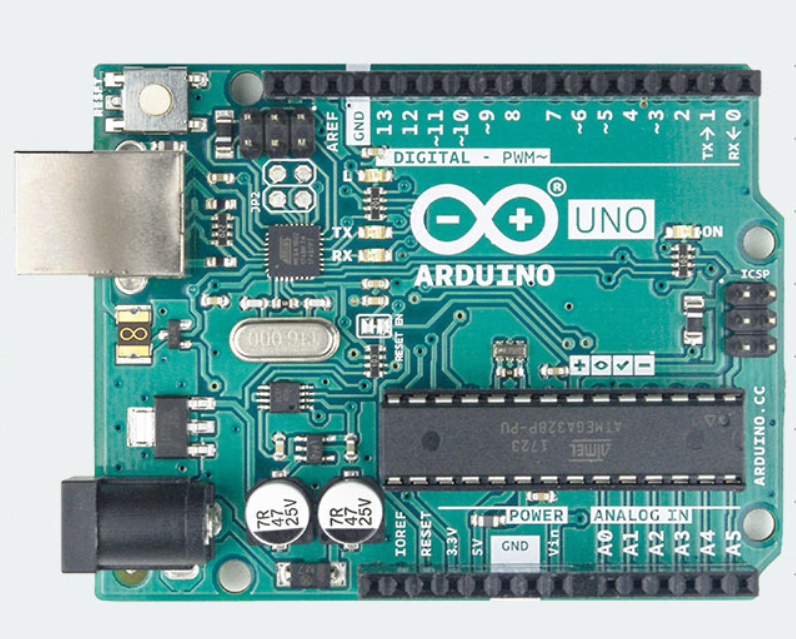
\includegraphics[height=5cm]{arduino.png}
    \bicaption[arduino UNO]{arduino UNO}{arduino UNO}
    \label{fig:arduino}
\end{figure}